\documentclass[12pt, a4paper]{article}
\renewcommand{\baselinestretch}{1.5}
\usepackage[toc,page]{appendix}
%\usepackage{mathptmx}
\usepackage[left=2cm,right=2cm, top=2cm, bottom=2cm]{geometry}
\usepackage{xcolor}
\usepackage{enumerate}
\usepackage{upgreek}
\usepackage{amssymb, amsmath, amsbsy}
\usepackage{subfigure} 
\usepackage[english]{babel}  % Caracteres en ESPAÑOL
\usepackage[utf8]{inputenc}
\usepackage{authblk}
\usepackage{graphicx}
\usepackage{mathrsfs}
\usepackage{hyperref}
\usepackage{apacite}
\usepackage[ruled,vlined]{algorithm2e}
\begin{document}
%%%%%%%%%%%%%%%%%%%%%%%%%%%%%%%%%%%%%%%%%%%%%%%%%%%%%%%%%%%%%%%%%%%%%%%%%%%%%%%%%%%%%%%%%%%%%%%%%%%%%%%%%%%%%%%%%%%%%%%%%%%%%%%%%%%%%%%%%%%%%%%%%%%%%%%%%%%%%%%%%%%%%%%%%%%%%%%%%%%%%
The model is solved by value function iteration based on the standard calibration of Arellano (2008)  considering 21 states for the output level, and 1000 grid points in the interval [-0.4:0] for debt. The computed value functions are:
\begin{figure}[!hbt]
	\centering
	\caption{Value function}
	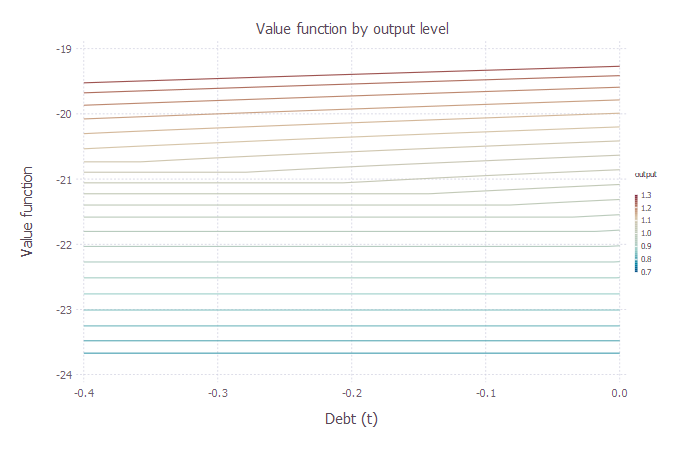
\includegraphics[scale=0.6, trim = 0 12 0 45, clip]{../Plots/ValuFunction.png}
	\begin{minipage}{0.65\textwidth}
	{\scriptsize The value functions are plotting by output level from blue [low level of output]  to red [high level of output].\par}
	\end{minipage}
\end{figure}
\\
The result shows states with high non-linearities. When we split the solution into the value of repayment and the value of default we find: \\
\begin{figure}[!hbt]
	\centering
	\caption{Value and Policy functions}
	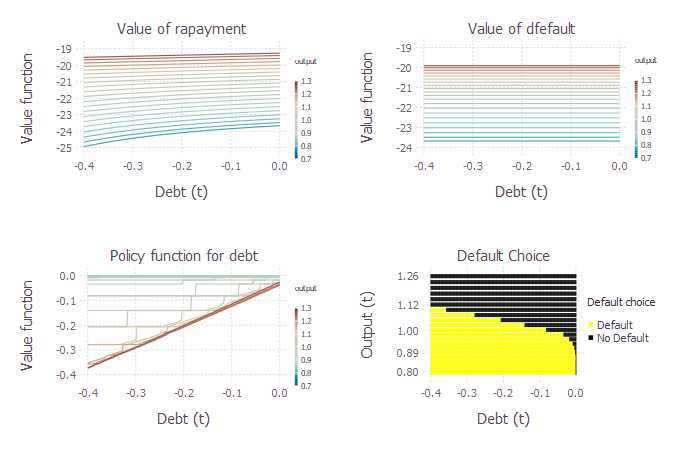
\includegraphics[scale=0.55,clip]{../Plots/Model0.png}
\end{figure}
\par In panels (a) and (b) I plot the value functions for repayment and default, respectively. Fo the latter, we observe linear function dependent of the state level. In contrast, the value of repayment is concave for low levels of production and passing to be almost linear in the high states. In panel (c) we observed that the policy function for new issued debt is highly non-linear, while the default choices (panel d) exhibits well defined limits between the states in which the government chooses whether defaulting.\\
\par After simulated 1 million observations (without burning anyone) from the model, I find a default probability of 2.7 percent with the following state of default (plotted in panel b):
\begin{figure}[!hbt]
	\centering
	\caption{Simulated default states}
	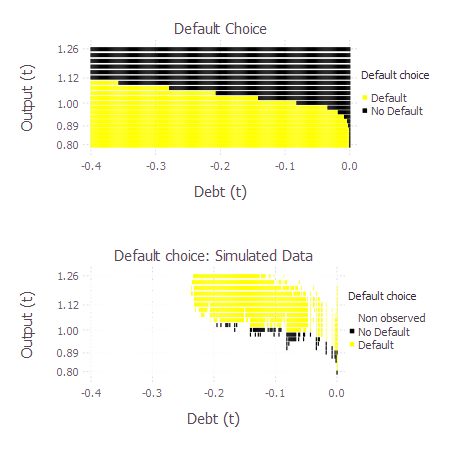
\includegraphics[scale=0.86]{../Plots/heat1.png}
	\begin{minipage}{0.65\textwidth}
		{\scriptsize Panel (b) plots the simulated states of default leaving in white the state combinations that are not observed in the simulation.\par}
	\end{minipage}
\end{figure}
The figure shows two potential problems that an implementation of a PLM could face. First, there is a large portion of the state-space that is not covered by the simulation. It could lead a high out-sample forecast problem given the overweight of non-default states. Then, I proceed to simulate 4 chains with the corners as initial states. This exercise does not solve the problem of small simulated data. For example, if we focus in the upper-left panel of figure 4 [when the simulation start in the lowest output level and higher debt state] we can observe that the optimal choice is defaulting. Therefore, in the next simulated period the government starts outside the market and without any debt moving to the observed region. Something similar happens in the low panel of figure 3. When the country starts with the highest level of output and debt its optimal decision is not defaulting but issuing less debt (lower-left panel of figure 4), the dynamics of the solution makes that in few steps the country arrives to the space of "observed data"
\begin{figure}[!hbt]
	\centering
	\caption{Simulated default states}
	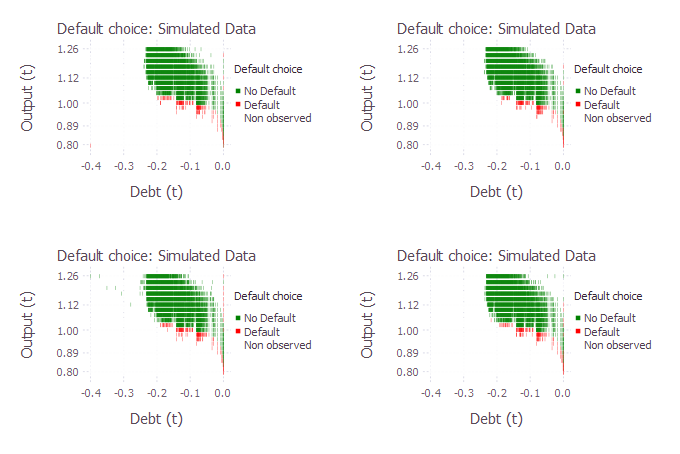
\includegraphics[scale=0.7]{../Plots/heats.png}
	\begin{minipage}{0.65\textwidth}
		{\scriptsize\par}
	\end{minipage}
\end{figure}
\\
Second, the difference between the policy function and the state of default. The policy function reflects the optimal default decision that government makes. However, we only observe that state of default which also considers stay in default after a defaulting. It is showed in panel (b) of figure 3  when although there is not debt the default state is still shaded in red.\\
Similar results are obtained if I apply the subroutine of markov chain simulation of Sargent downloaded from QuantEcon.
\begin{figure}[!hbt]
	\centering
	\caption{Simulated default states (QuantEcon Simulation)}
	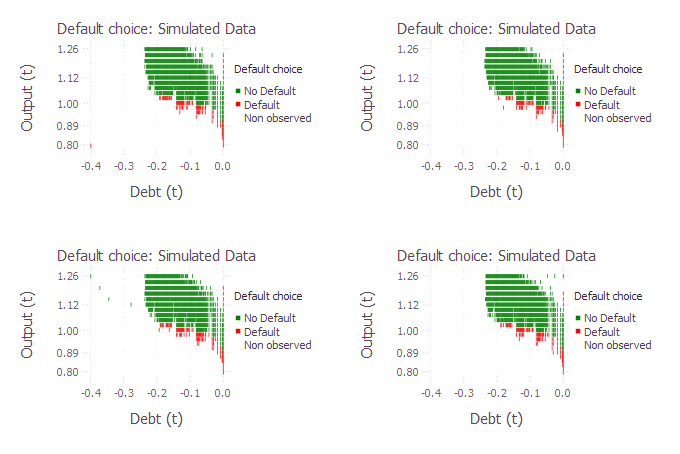
\includegraphics[scale=0.7]{../Plots/heats(Quant).png}
	\begin{minipage}{0.65\textwidth}
		{\scriptsize\par}
	\end{minipage}
\end{figure}
\section{The updating algorithm}
To update the policy functions, I follow: \\
\begin{algorithm}[H]
%	\SetAlgoLined
	\textbf{Initialization : $v_{r}^{(0)}, v_{d}^{(0)}$}\\
		$v^{(0)} = max\left(v_{r}^{(0)}, v_{d}^{(0)}\right)$ \\
	\textbf{Initial bond price:} \\
	$D^{(0)} = \mathcal{I} \left(max\left(v_{r}^{(0)}, v_{d}^{(0)}\right)\right)$\\
	$\delta^{(0)} = D^{(0)} \Pi^T$\\
	$q^{(0)} = \left(\frac{1}{1-r}\right) .* (1 \, .- \delta^{(0)})$ \\
	\textbf{Updating expectations:} \\
	$\mathbb{E}[v]^{(1)} = v^{(0)} \Pi^T$\\
	$\mathbb{E}[v_{r}]^{(1)} = v^{(0)}_{r} \Pi^T$\\
	$\mathbb{E}[v_{d}]^{(1)} = v^{(0)}_{d} \Pi^T$\\
	\textbf{Finding Policy function and updating value functions (and price):} \\
	$v_r^{(1)} = max\{ u(b+y - q^{(0)}b') + \beta\mathbb{E}[v]^{(1)} \} \rightarrow \text{by choosing } b^{(1)'}$ \\
	$v_d^{(1)} = u(y^{def}) + \beta(\theta \mathbb{E}[v| b'=0]^{(1)} + (1-\theta)\mathbb{E}[v_d]^{(1)})$\\
	$v^{(1)} = max\left(v_{r}^{(1)}, v_{d}^{(1)}\right)$ \\
	$D^{(1)} = \mathcal{I} \left(max\left(v_{r}^{(1)}, v_{d}^{(1)}\right)\right)$\\
	$\delta^{(1)} = D^{(1)} \Pi^T$\\
	$q^{(1)} = \left(\frac{1}{1-r}\right) .* (1 \, .- \delta^{(1)})$ \\
%	\caption{algorithms}
\end{algorithm}
To verify that the implementation is correct I run the algorithm with the value functions solved in the model and I find no discrepancy in the updated policy functions\\
\section{Selecting initial models}
Before to implement the algorithm with simulated data, I will show how some model perform when they use all the information from the model [value functions in the whole grid]. The models to be compare are:
\begin{enumerate}
	\item OLS:
		$$
		v_r = \beta_0 + \beta_1b + \beta_2 y+ \beta_3b^2 + \beta_4y^2 +\beta_5 b* y + \epsilon
		$$
	\item Power series with normalization in range [-1,1]: \\If x lies in the interval [a,b], the transformation:
		$$\tilde x =2\frac{x- a}{b-a} - 1 $$  will lies in the interval [-1,1].\\
	Procedure:
	\begin{itemize}
		\item Determine an expansion degree $d$
		\item I calculate $\tilde b$, $\tilde y$ , and  $\tilde v_r$
		\item Estimate by OLS
		$$
		 \tilde v_r = \sum_{i=0}^d\sum_{j=0}^{d-i} \alpha_{i,j}\tilde b^{i} \tilde y^{j} +\epsilon_{ps}
		$$
	\end{itemize}	
	\item Chebyshev basis: Procedure
		\begin{itemize}
		\item Determine an expansion degree $d$
		\item I calculate $\tilde b$, $\tilde y$ , and  $\tilde v_r$
		\item Estimate by OLS
		$$
		 \tilde v_r = \sum_{i=0}^d\sum_{j=0}^{d-i} \theta_{i,j}T_i(\tilde b) T_j(\tilde y^{j})+ +\epsilon_{cheb}
		$$
		where $T(x)$ is the Chebyshev polynomial of the first kind.
		\end{itemize}	
	\item Neural Networks with one hidden layer, 16 neurons and the following activation functions
	\begin{enumerate}
		\item softplus: \hspace{1mm}$f(x) = log(exp(x) + 1)$ 
		\item tanh:\hspace{8mm}$f(x) = \frac{exp(2x)-1}{exp(2x)+1}$
		\item elu: \hspace{9mm}$f(x) = \begin{cases}
			x   \quad \quad \quad\quad\quad \text{if} \quad x >0\\
			exp(x) -1 \quad \text{otherwise}
		\end{cases}$
		\item sigmoid:\hspace{2mm}$f(x) = \frac{1}{1+exp(-x)}$
		\item swish: \hspace{4mm}$f(x) = \frac{x}{1+exp(-x)}$
	\end{enumerate}
	The estimation is made by using a descent algorithm,and minimizing the MSE. Each sample is composed by 10 times the total observations number randomly sorted to exploit the learning. I also interpolate linearly 3 points between each original debt point. I consider 10 epochs per model training. 
\end{enumerate}
Table \ref{tab:1} show the MSE and MAE calculated  over the original values of $v_r$ after estimating each model with $d=4$\\
\begin{table}[!hbt]
	\centering
	\caption{Fit error by model}
	\vspace{3mm}
	\begin{tabular}{|c|cccccccc|}
		\hline
		   & OLS&Power series& Chebyshev&Sotfplus&Tanh&Elu&Sigmoid&Swish\\
		\hline
		RMSE& 0.034&	0.009&	0.009&	0.012&	0.007&	0.008&	0.01&	0.011 \\
		MAE& 0.149&	0.03&	0.03&	0.037&	0.026&	0.028&	0.033&	0.039\\
		RMS $100*\frac{\hat v_r -v_r}{v_r}$ &0.155&	0.04&	0.04&	0.053&	0.033&	0.035&	0.045&	0.051	\\
		MA  $100*\frac{\hat v_r -v_r}{v_r}$ &0.604&	0.125&	0.125&	0.186&	0.121&	0.112&	0.167&	0.165\\
		\hline
	\end{tabular}
	\label{tab:1}
\end{table}
\begin{figure}[!hbt]
	\centering
	\caption{Estimated residual}
	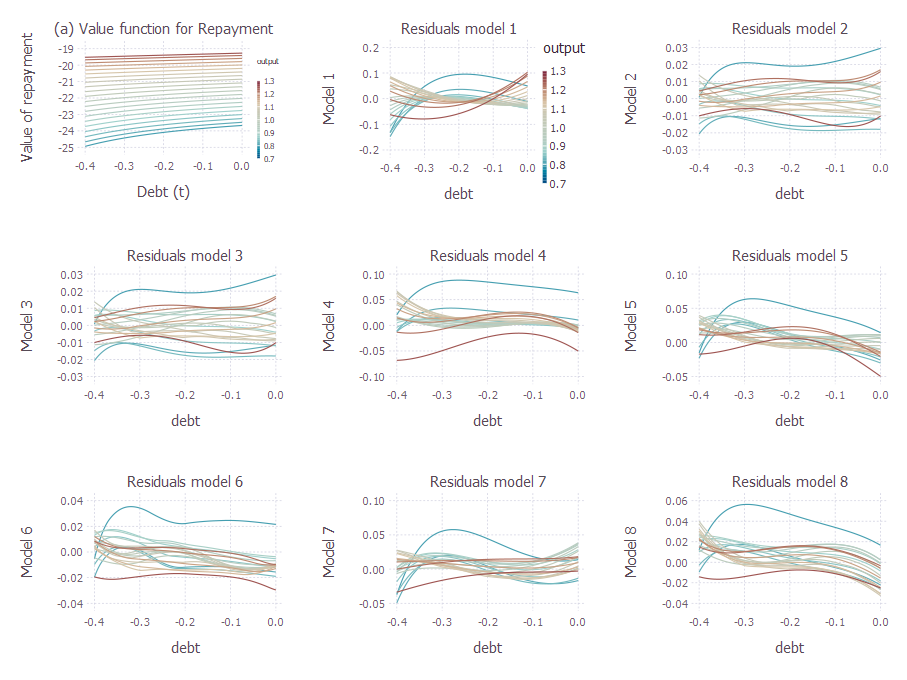
\includegraphics[scale=0.5]{../Plots/res1.png}
	\begin{minipage}{0.85\textwidth}
	{\scriptsize Panel (a)  plots the value of repayment, while the rest of panel plot the residuals of each proposed model.\par}
	\end{minipage}
\end{figure}
\par In relative terms, there are not big differences between power series functions and neural networks, but after applying the updating algorithm and simulated 1oo thousands observations, I find high volatility in terms of percentage of defaults.
\begin{table}[!hbt]
	\centering
	\caption{Fit error by model}
	\vspace{3mm}
	\begin{tabular}{|c|cccccccc|}
		\hline
		& OLS&Power series& Chebyshev&Sotfplus&Tanh&Elu&Sigmoid&Swish\\
		\hline
		Default \%&  8.2 & 1.9 & 1.9 & 15 & 32 & 28 & 21 & 0.2 \\
		\% Default Error& 2.7 & 0.4 & 0.4 &0.6& 0.3&0.2&0.6&0.32\\
		\hline
	\end{tabular}
	\label{tab:1}
\end{table}
With exception of the simplest OLS model, the percentage of error in default decisions are lower than 2 percent. However, the OLS model performs better in one-step ahead updating. 
\par One possible explanation of these results appears after observing the error in the policy function for  new debt after updating. Figure \ref{fig:erroPF} plots these series.
\begin{figure}[!hbt]
	\centering
	\caption{Estimated Debt Policy functions}
	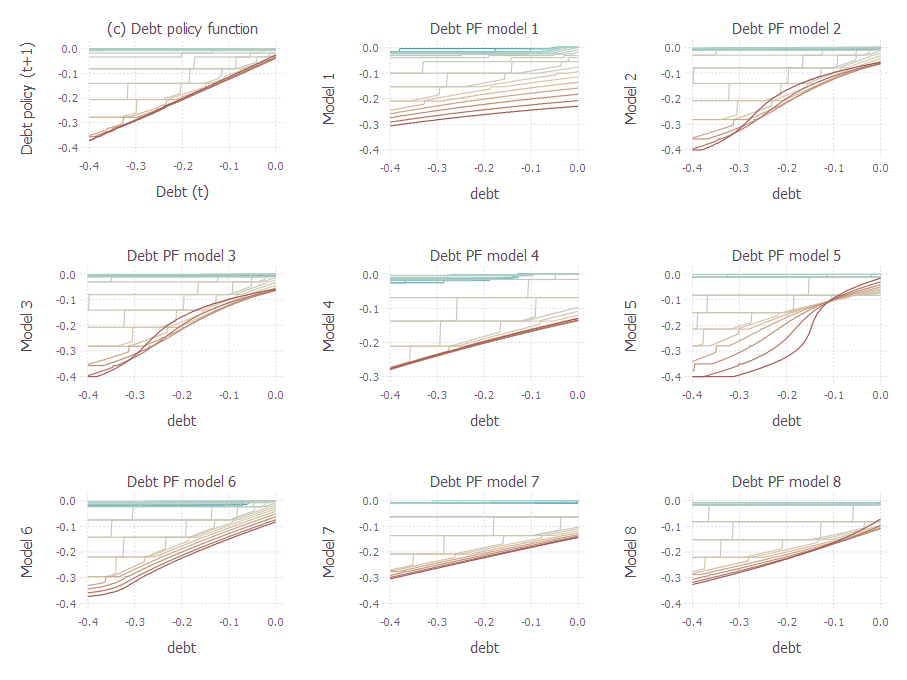
\includegraphics[scale=0.5]{../Plots/PFB.png}
	\begin{minipage}{0.85\textwidth}
		{\scriptsize Panel (a)  plots the policy function for debt, while the rest of panels plot the policy function for new debt of each proposed model.\par}
	\end{minipage}
\end{figure}

\begin{figure}[!hbt]
	\centering
	\caption{Error in Policy functions}
	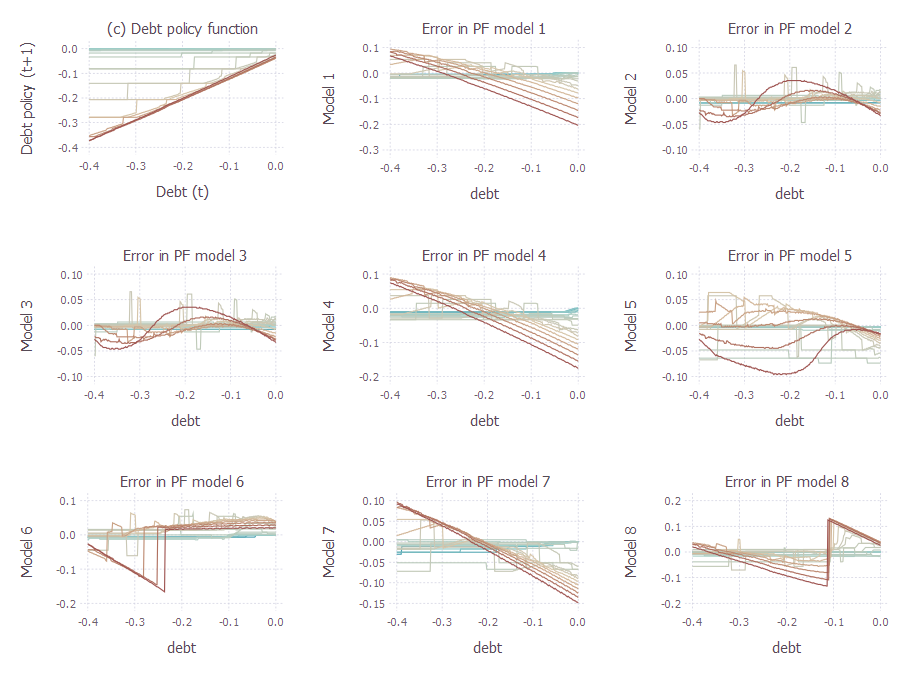
\includegraphics[scale=0.5]{../Plots/PFBerror.png}
	\begin{minipage}{0.85\textwidth}
		{\scriptsize Panel (a)  plots the policy function for debt, while the rest of panels plot the residuals of each proposed model.\par}
	\end{minipage}
	\label{fig:erroPF}
\end{figure}
%%%%%%%%%%%%%%%%%%%%%%%%%%%%%%%%%%%%%%%%%%%%%%%%%%%%%%%%%%%%%%%%%%%%%%%%%%%%%%%%%%%%%%%%%%%%%%%%%%%%%%%%%%%%%%%%%%%%%%%%%%%%%%%%%%%%%%%%%%%%%%%%%%%%%%%%%%%%%%%%%%%%%%%%%%%%%%%%%%%%%
\end{document}